%=================================================
\chapter{Inventory Analysis \& Document Restructuring (Point 1)}
%=================================================

\section{Overview}

This phase establishes a clear inventory of all legacy assets and
restructures documentation so that subsequent reengineering work (reverse
engineering, code restructuring, data restructuring, and forward
engineering) can be carried out in a disciplined, traceable way.

The legacy system is a Java Swing--based Point-of-Sale (POS) application
for SG Technologies, backed by multiple plain-text files. In addition, a
forward-engineered Node.js API and migration utilities already exist in
the codebase.

\begin{figure}[h]
  \centering
  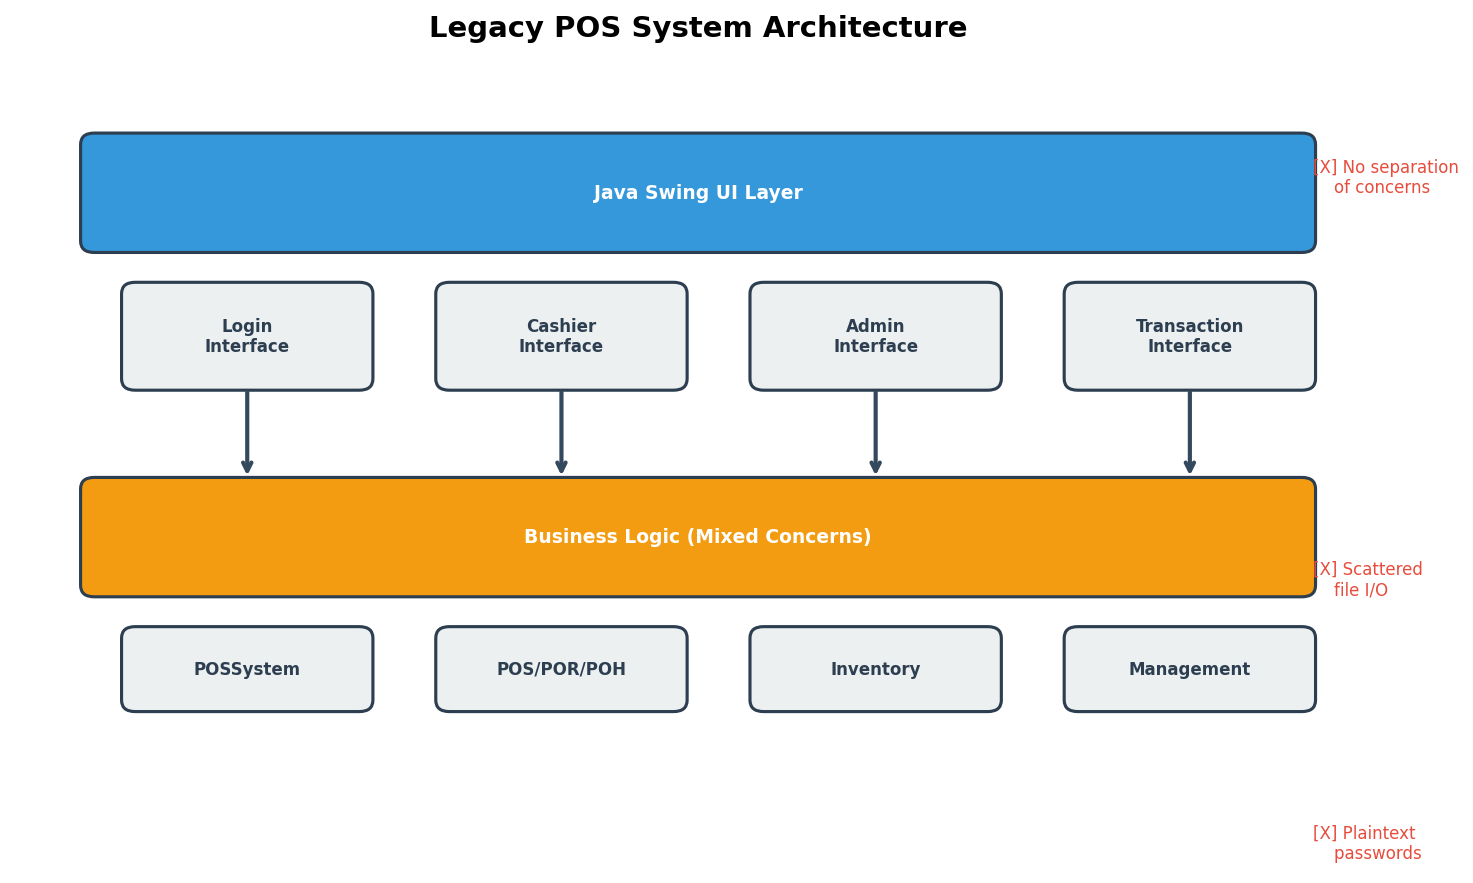
\includegraphics[width=0.85\textwidth]{images/legacy_system_overview.png}
  \caption{Legacy System Overview -- Java Swing desktop application with
           direct file-based persistence using plain text files.}
  \label{fig:legacy-overview}
\end{figure}

\section{Asset Inventory}

Based on the legacy code base and project directories, the main assets
are:

\subsection*{Code (Legacy Java)}

\begin{itemize}[leftmargin=1.2cm]
  \item \textbf{UI Layer}
  \begin{itemize}
    \item \texttt{src/Login\_Interface.java}
    \item \texttt{src/Cashier\_Interface.java}
    \item \texttt{src/Admin\_Interface.java}
    \item \texttt{src/Transaction\_Interface.java}
  \end{itemize}
  \item \textbf{Business Logic}
  \begin{itemize}
    \item \texttt{src/PointOfSale.java}
    \item \texttt{src/POS.java}
    \item \texttt{src/POR.java}
    \item \texttt{src/POH.java}
    \item \texttt{src/POSSystem.java}
    \item \texttt{src/Inventory.java}
    \item \texttt{src/Management.java}
    \item \texttt{src/EmployeeManagement.java}
    \item \texttt{src/Item.java}
    \item \texttt{src/Employee.java}
  \end{itemize}
  \item \textbf{Duplicated Code Trees}
  \begin{itemize}
    \item Duplicated copies under \texttt{src/src/...} (interfaces and
          business logic), to be treated as obsolete duplicates.
  \end{itemize}
\end{itemize}

\subsection*{Data Files (Plain Text)}

\begin{itemize}[leftmargin=1.2cm]
  \item Inventory:
        \texttt{Database/itemDatabase.txt},
        \texttt{Database/rentalDatabase.txt}
  \item Employees:
        \texttt{Database/employeeDatabase.txt}
  \item Rentals/Customers:
        \texttt{Database/userDatabase.txt}
  \item Sales invoices:
        \texttt{Database/saleInvoiceRecord.txt}
  \item Temporary/intermediate:
        \texttt{Database/newTemp.txt},
        \texttt{Database/newEmployeeDatabase.txt}
\end{itemize}

\subsection*{Forward-Engineered Code (Node.js)}

\begin{itemize}[leftmargin=1.2cm]
  \item API:
        \texttt{forward-engineered/api/index.js},
        routers under \texttt{forward-engineered/api/routes/*},
        models under \texttt{forward-engineered/api/models/*}
  \item Config:
        \texttt{forward-engineered/api/.env}
        (contains \texttt{MONGODB\_URI}; secrets not committed)
  \item Migration utilities:
        \texttt{forward-engineered/migration/index.js},
        \texttt{forward-engineered/migration/package.json}
\end{itemize}

\section{Classification of Assets}

Each asset is categorised as \emph{active}, \emph{obsolete}, or
\emph{reusable} for forward engineering. Table~\ref{tab:asset-classification}
provides a complete classification summary.

\begin{table}[h]
  \centering
  \caption{Complete Asset Classification}
  \label{tab:asset-classification}
  \begin{tabular}{p{4cm} p{4.5cm} p{2cm} p{2.5cm}}
    \toprule
    \textbf{Asset} & \textbf{Location} & \textbf{Status} & \textbf{Action} \\
    \midrule
    Login\_Interface.java & src/ & Active & Reengineer \\
    Cashier\_Interface.java & src/ & Active & Reengineer \\
    Admin\_Interface.java & src/ & Active & Reengineer \\
    Transaction\_Interface.java & src/ & Active & Reengineer \\
    POSSystem.java & src/ & Active & Reengineer \\
    PointOfSale.java & src/ & Active & Reengineer \\
    POS.java & src/ & Active & Reengineer \\
    POR.java & src/ & Active & Reengineer \\
    POH.java & src/ & Active & Reengineer \\
    Inventory.java & src/ & Active & Reengineer \\
    Item.java & src/ & Reusable & Reference \\
    Employee.java & src/ & Reusable & Reference \\
    \midrule
    src/src/* duplicates & src/src/ & Obsolete & Delete \\
    newTemp.txt & Database/ & Obsolete & Delete \\
    newEmployeeDatabase.txt & Database/ & Obsolete & Delete \\
    \midrule
    itemDatabase.txt & Database/ & Reusable & Migrate \\
    employeeDatabase.txt & Database/ & Reusable & Migrate \\
    userDatabase.txt & Database/ & Reusable & Migrate \\
    rentalDatabase.txt & Database/ & Reusable & Migrate \\
    saleInvoiceRecord.txt & Database/ & Reusable & Migrate \\
    \bottomrule
  \end{tabular}
\end{table}

\subsection*{Active (Legacy)}

\begin{itemize}[leftmargin=1.2cm]
  \item Core transactional and management classes:
        \texttt{PointOfSale}, \texttt{POS}, \texttt{POR}, \texttt{POH},
        \texttt{POSSystem}, \texttt{Inventory}, \texttt{Management},
        \texttt{EmployeeManagement}, \texttt{Transaction\_Interface}.
\end{itemize}

\subsection*{Obsolete or Duplicate}

\begin{itemize}[leftmargin=1.2cm]
  \item \texttt{src/src/interfaces/*} and \texttt{src/src/bl/*} as
        duplicates of legacy classes; to be consolidated into a single
        \texttt{src/} tree.
  \item Temporary DB files:
        \texttt{Database/newTemp.txt} and
        \texttt{Database/newEmployeeDatabase.txt}.
\end{itemize}

\subsection*{Reusable for Forward Engineering}

\begin{itemize}[leftmargin=1.2cm]
  \item Legacy data files under \texttt{Database/*} as sources for
        migration into a structured database.
  \item Domain concepts in Java classes \texttt{Item} and \texttt{Employee}
        as references when designing new database schemas and models.
  \item Existing forward-engineered API and migration scripts under
        \texttt{forward-engineered/*}.
\end{itemize}

\section{Legacy Code Examples}

The following code examples demonstrate the structure of key legacy components
that were analyzed during the inventory phase.

\subsection{Employee Data Model (Legacy)}

\begin{lstlisting}[language=Java]
// src/Employee.java - Legacy employee class
public class Employee {
    private String employeeId;
    private String firstName;
    private String lastName;
    private String role;        // "Admin" or "Cashier"
    private String password;    // PLAINTEXT - Security issue!
    
    public Employee(String id, String role, String first, String last, String pass) {
        this.employeeId = id;
        this.role = role;
        this.firstName = first;
        this.lastName = last;
        this.password = pass;   // Stored as-is
    }
    
    // Getters and setters...
}
\end{lstlisting}

\subsection{Inventory Access (Legacy)}

\begin{lstlisting}[language=Java]
// src/Inventory.java - Direct file access pattern
public class Inventory {
    private ArrayList<Item> items = new ArrayList<>();
    
    public void loadItems() {
        try {
            FileReader fr = new FileReader("Database/itemDatabase.txt");
            BufferedReader br = new BufferedReader(fr);
            String line;
            
            while ((line = br.readLine()) != null) {
                String[] parts = line.split(" ");
                int id = Integer.parseInt(parts[0]);
                String name = parts[1];
                double price = Double.parseDouble(parts[2]);
                int quantity = Integer.parseInt(parts[3]);
                
                items.add(new Item(id, name, price, quantity));
            }
            br.close();
        } catch (IOException e) {
            e.printStackTrace();  // Poor error handling
        }
    }
}
\end{lstlisting}

\section{Dependency Map (Legacy)}

The dependency map clarifies how UI, business, and persistence layers
interact.

\begin{figure}[h]
  \centering
  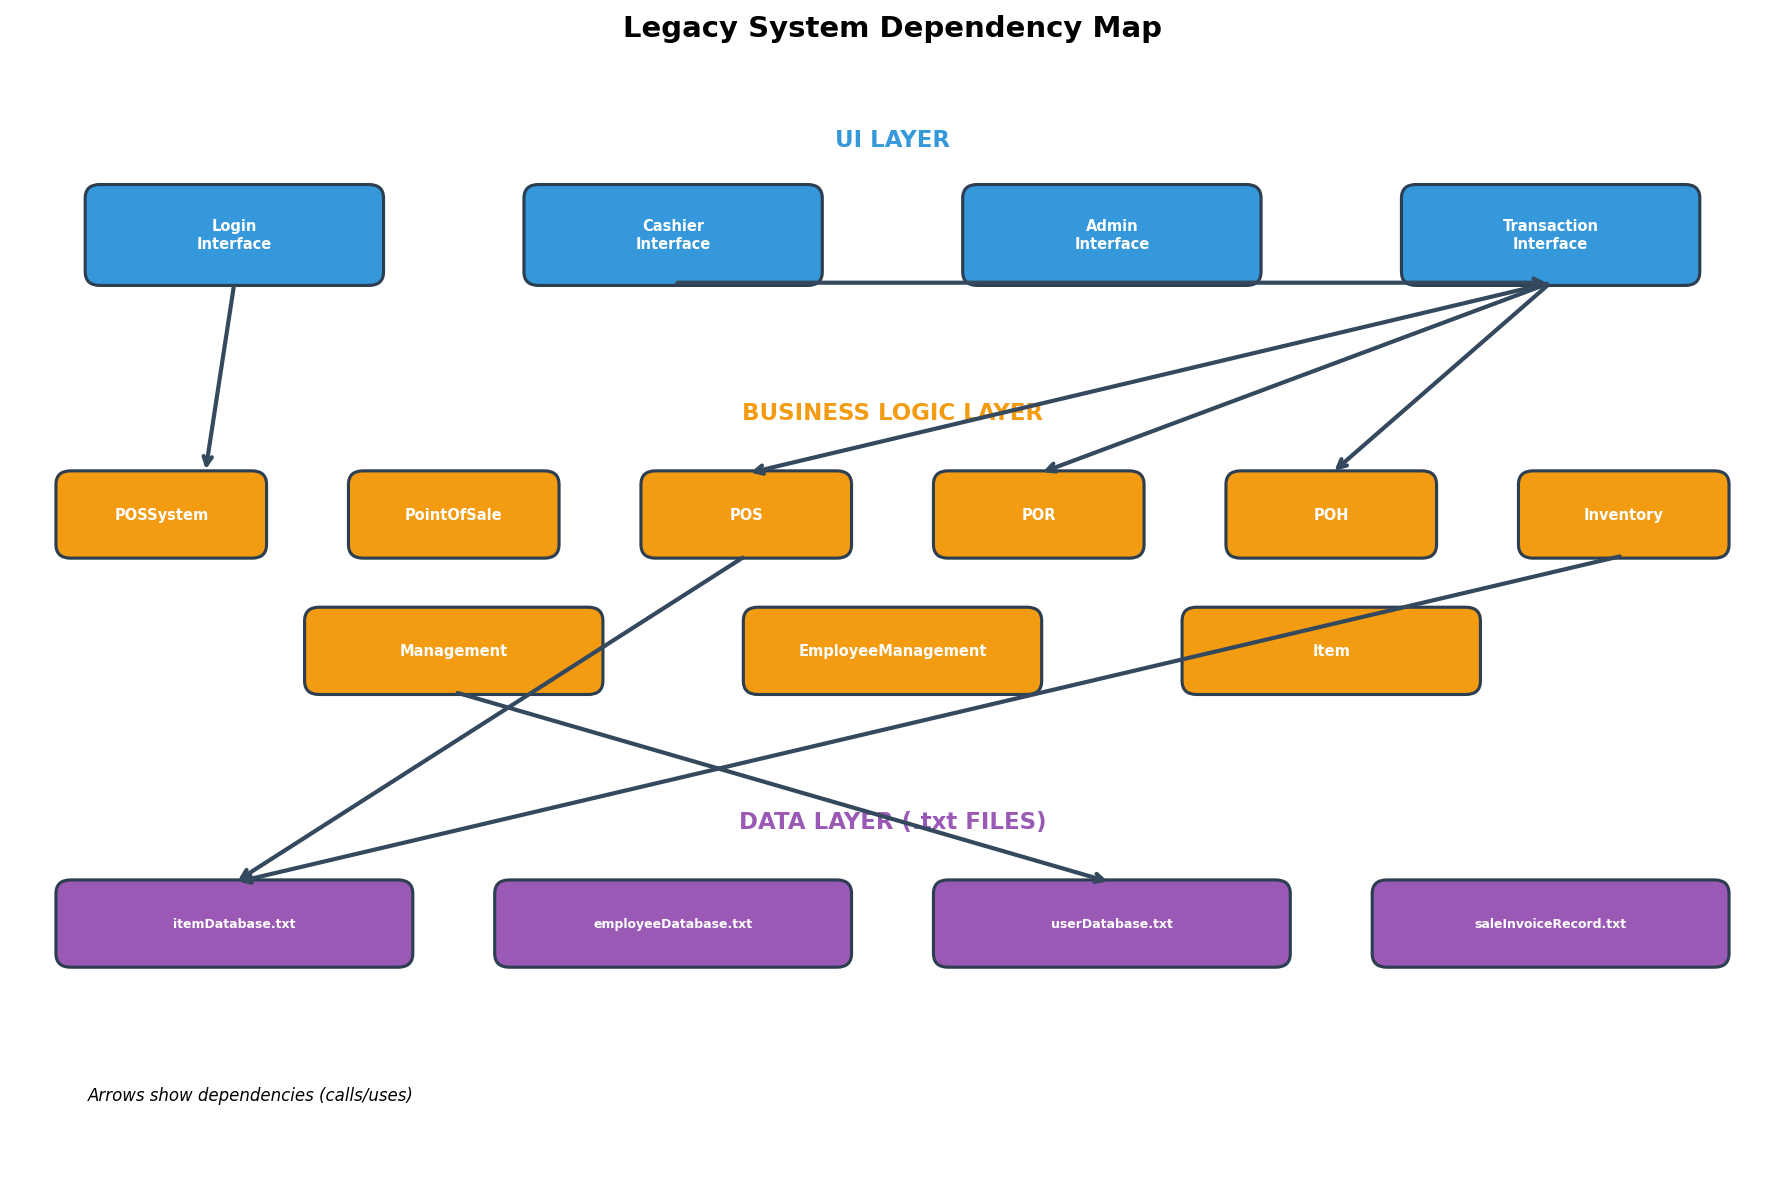
\includegraphics[width=0.95\textwidth]{images/legacy_dependency_map.png}
  \caption{Legacy System Dependency Map -- Shows the relationships between UI classes,
           business logic components, and text file data storage in the original
           Java Swing POS application.}
  \label{fig:legacy-dependency-map}
\end{figure}

\subsection*{UI to Business}

\begin{itemize}[leftmargin=1.2cm]
  \item \texttt{Login\_Interface.java} calls
        \texttt{POSSystem.logIn(...)} (e.g., \texttt{src/POSSystem.java:166}).
  \item \texttt{Cashier\_Interface.java} launches
        \texttt{Transaction\_Interface} based on the selected operation
        (Sale/Rental/Return).
  \item \texttt{Admin\_Interface.java} interacts with
        \texttt{EmployeeManagement}.
\end{itemize}

\subsection*{Business to Persistence}

\begin{itemize}[leftmargin=1.2cm]
  \item \texttt{PointOfSale.java} orchestrates transactions, starting
        with inventory access.
  \item \texttt{POS.java} writes sales invoices (\texttt{Total with tax})
        to \texttt{saleInvoiceRecord.txt}.
  \item \texttt{POR.java} and \texttt{POH.java} handle rentals and
        late-fee computations.
  \item \texttt{Inventory.java} reads and updates
        \texttt{itemDatabase.txt}.
  \item \texttt{Management.java} appends rental entries to
        \texttt{userDatabase.txt}.
\end{itemize}

\section{Document Restructuring Plan}

To support team hand-off and future maintenance, documentation is
restructured into phase-focused files under \texttt{docs/}:

\begin{itemize}[leftmargin=1.2cm]
  \item \texttt{docs/01-inventory-and-document-restructuring.md}
  \item \texttt{docs/02-reverse-engineering-and-smell-detection.md}
  \item \texttt{docs/03-code-restructuring.md}
  \item \texttt{docs/04-data-restructuring-and-migration.md}
\end{itemize}

Code references are documented using
\texttt{file\_path:line\_number} notation to ensure precise traceability
from narrative documentation to actual source lines.

%=================================================
\chapter{Reverse Engineering \& Smell Detection (Point 2)}
%=================================================

\section{Extracted Architecture and Workflows}

Reverse engineering was applied to extract the runtime behaviour and
architecture of the legacy system.

\begin{figure}[h]
  \centering
  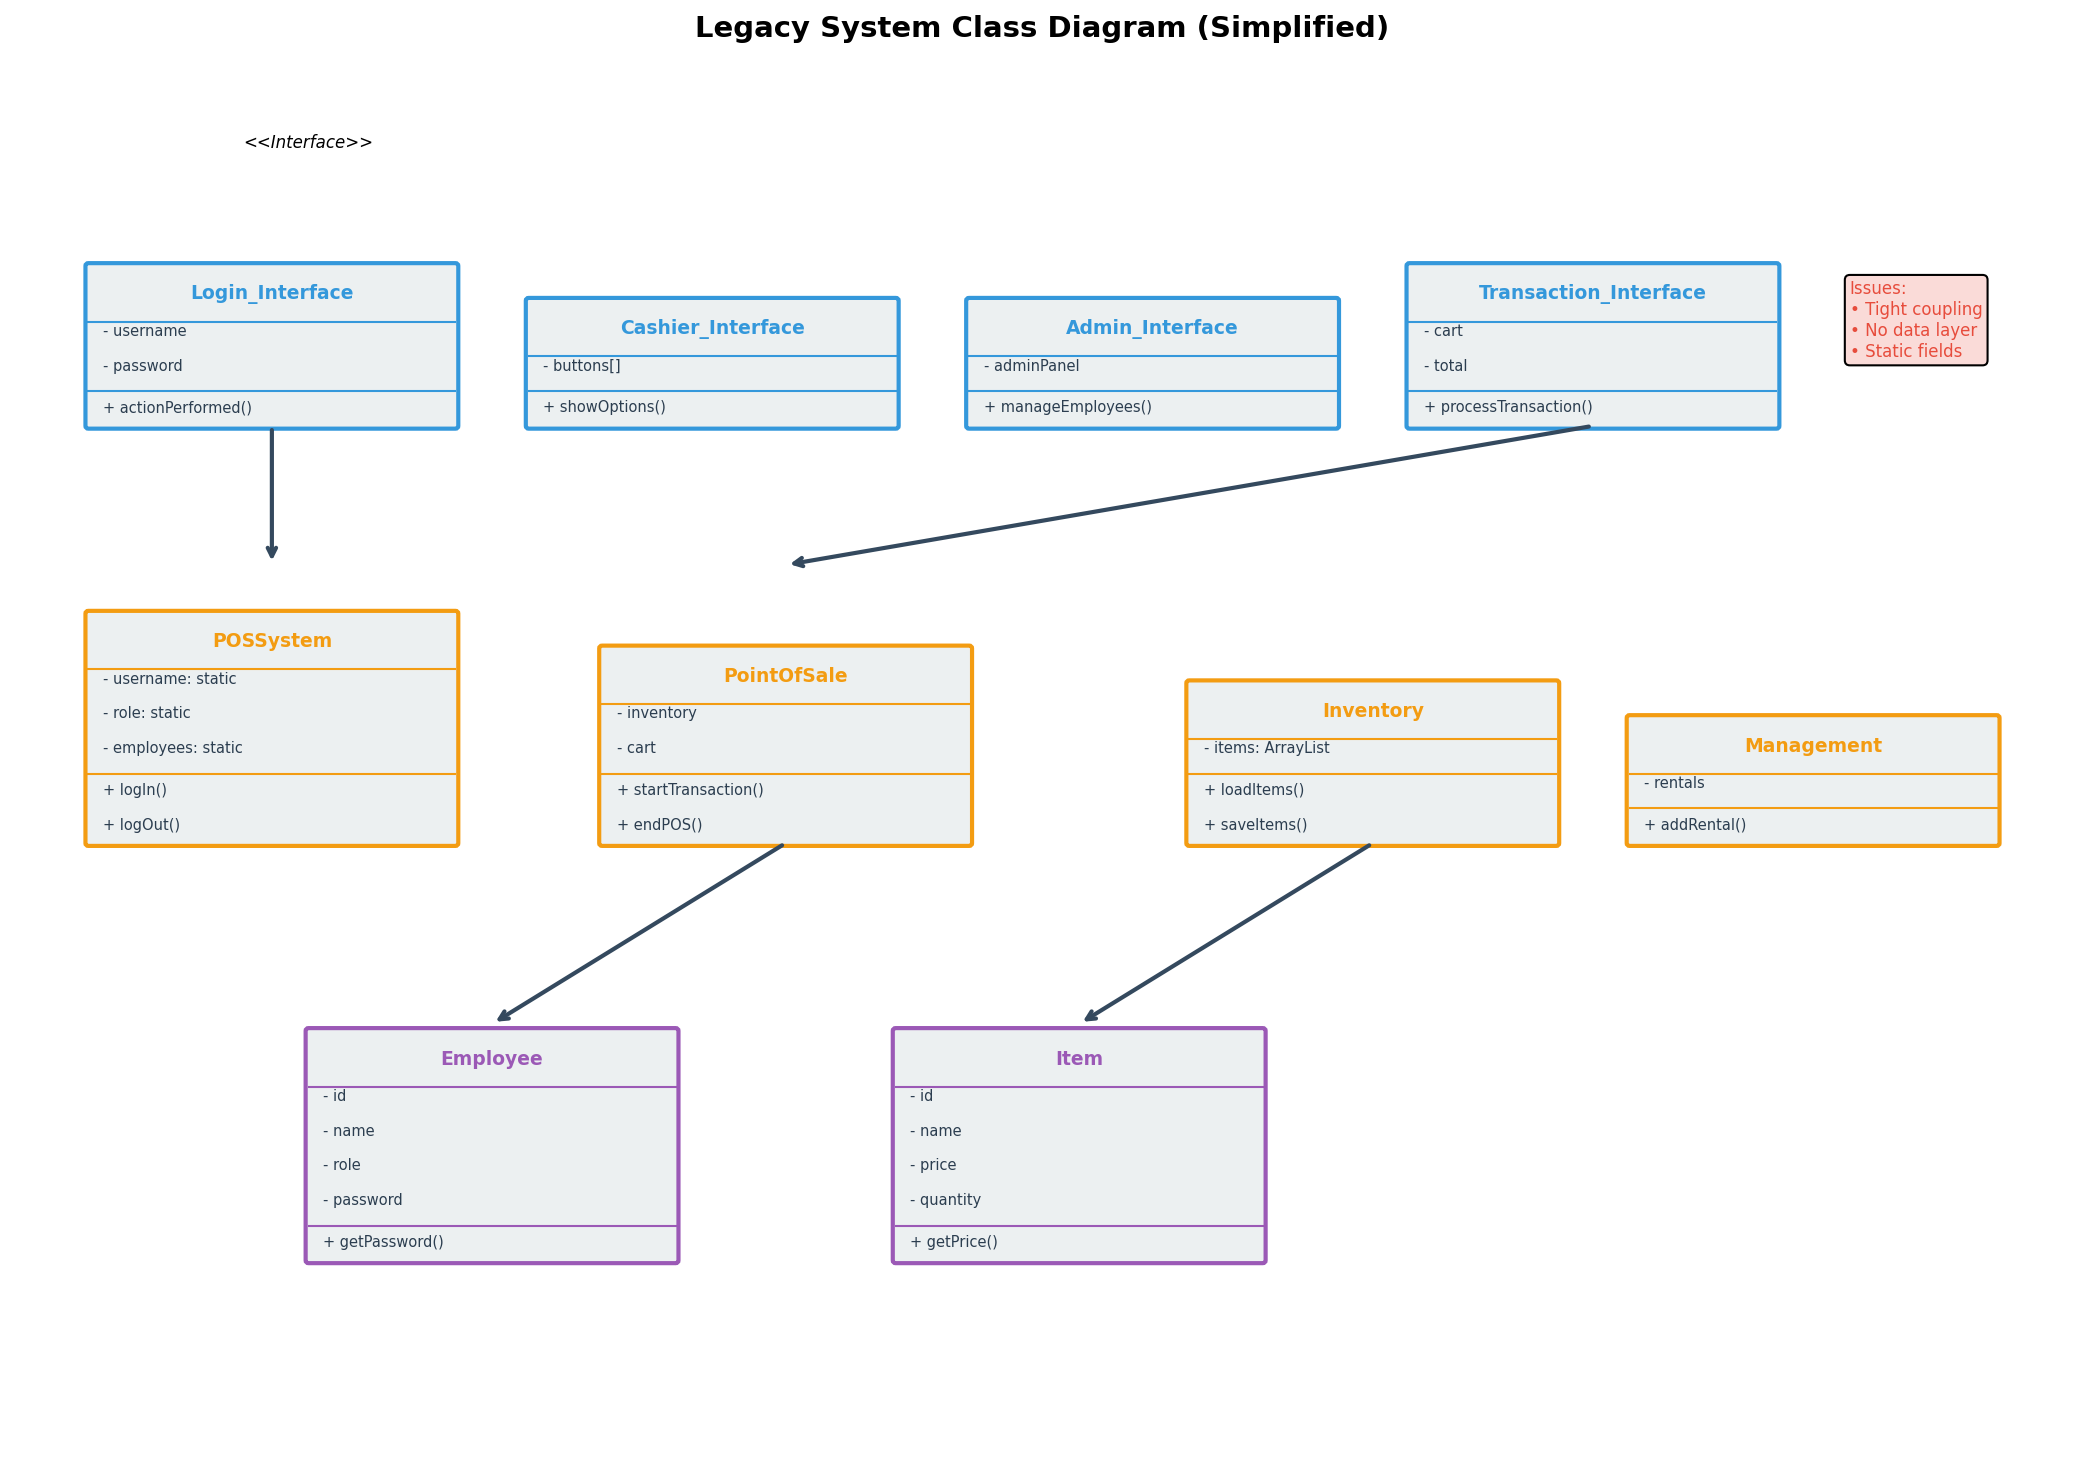
\includegraphics[width=0.95\textwidth]{images/legacy_class_diagram.png}
  \caption{Legacy System Class Diagram -- Extracted class structure showing UI interfaces,
           business logic classes, and data models. Note the tight coupling between
           UI and business logic, and the absence of a data access layer.}
  \label{fig:legacy-class-diagram}
\end{figure}

\subsection*{Login Flow}

\begin{itemize}[leftmargin=1.2cm]
  \item \texttt{Login\_Interface.java} authenticates users via
        \texttt{POSSystem.logIn(...)}.
  \item Role (Cashier/Admin) determines the next user interface screen.
\end{itemize}

\subsection*{Cashier Workflow}

\begin{itemize}[leftmargin=1.2cm]
  \item \texttt{Cashier\_Interface.java} triggers
        \texttt{Transaction\_Interface} with an operation flag:
        \emph{Sale}, \emph{Rental}, or \emph{Return}.
\end{itemize}

\subsection*{Transaction Workflow}

\begin{itemize}[leftmargin=1.2cm]
  \item \texttt{Transaction\_Interface.java} selects
        \texttt{POS} (sales), \texttt{POR} (rental), or
        \texttt{POH} (returns), and sets the underlying database file
        accordingly.
  \item \texttt{PointOfSale.java} initialises with inventory, builds the
        cart, and delegates to operation-specific methods (e.g.,
        \texttt{endPOS}).
\end{itemize}

\subsection*{Persistence Responsibilities}

\begin{itemize}[leftmargin=1.2cm]
  \item Inventory: \texttt{Inventory.java} reads and writes inventory
        text files.
  \item Employees: \texttt{EmployeeManagement.java} updates employee
        records and rewrites the file.
  \item Rentals/Customers: \texttt{Management.java} appends rental
        entries to \texttt{Database/userDatabase.txt}.
  \item Sales: \texttt{POS.java} writes item lines and a final
        \texttt{Total with tax} line to \texttt{saleInvoiceRecord.txt}.
\end{itemize}

\section{Code Smells (Examples)}

Several critical code smells were identified during reverse engineering.
Table~\ref{tab:code-smells} summarizes the findings with evidence.

\begin{table}[h]
  \centering
  \caption{Code Smells Identified with Evidence}
  \label{tab:code-smells}
  \begin{tabular}{p{1cm} p{3.5cm} p{4cm} p{4.5cm}}
    \toprule
    \textbf{ID} & \textbf{Smell} & \textbf{Location} & \textbf{Evidence} \\
    \midrule
    CS1 & Duplicated Source Trees & \texttt{src/} and \texttt{src/src/} & Identical classes in both directories \\
    CS2 & Scattered File I/O & Multiple classes & 8+ classes with direct FileReader/Writer \\
    CS3 & Magic Numbers & \texttt{POH.java:71} & Hardcoded \texttt{0.1} for late fee rate \\
    CS4 & Global Mutable State & \texttt{POSSystem.java} & Static fields for username, role, etc. \\
    CS5 & Plaintext Passwords & \texttt{POSSystem.java:166} & Direct string comparison for auth \\
    CS6 & Poor Error Handling & Multiple classes & \texttt{e.printStackTrace()} only \\
    CS7 & God Class & \texttt{POSSystem.java} & 400+ lines, handles auth + state + utils \\
    \bottomrule
  \end{tabular}
\end{table}

\subsection{CS3: Magic Numbers Evidence}

\begin{lstlisting}[language=Java]
// src/POH.java:71 - Hardcoded late fee rate
public void calculateLateFee() {
    // Magic number 0.1 = 10% per day late fee
    itemPrice = amount * price * 0.1 * days;  // What does 0.1 mean?
    
    // Another magic number for tax
    totalPrice = totalPrice * 1.06;  // 6% tax hardcoded
}
\end{lstlisting}

\subsection{CS4: Global Mutable State Evidence}

\begin{lstlisting}[language=Java]
// src/POSSystem.java - Global mutable state (anti-pattern)
public class POSSystem {
    // Static mutable fields - shared across ALL instances
    public static String username;
    public static String password;
    public static String name;
    public static String role;
    public static ArrayList<Employee> employees;
    
    // Any class can modify these at any time!
    public static void setRole(String r) { role = r; }
}
\end{lstlisting}

\subsection{CS5: Plaintext Password Evidence}

\begin{lstlisting}[language=Java]
// src/POSSystem.java:166 - CRITICAL SECURITY VULNERABILITY
public static boolean logIn(String user, String pass) {
    for (Employee emp : employees) {
        if (emp.getId().equals(user)) {
            // Direct string comparison - password stored in PLAINTEXT!
            if (emp.getPassword().equals(pass)) {
                username = user;
                password = pass;  // Storing plaintext password in memory
                role = emp.getRole();
                return true;
            }
        }
    }
    return false;
}
\end{lstlisting}

\subsection{CS6: Poor Error Handling Evidence}

\begin{lstlisting}[language=Java]
// src/Inventory.java - Poor error handling pattern
public void updateQuantity(int itemId, int delta) {
    try {
        FileWriter fw = new FileWriter("Database/itemDatabase.txt");
        // ... file operations
    } catch (IOException e) {
        e.printStackTrace();  // Just prints to console!
        // No user notification
        // No rollback
        // No logging
        // Application continues in unknown state
    }
}
\end{lstlisting}

\section{Data Smells (Examples)}

Inspection of the text databases revealed several data-quality issues.
Table~\ref{tab:data-smells} provides a summary of findings.

\begin{table}[h]
  \centering
  \caption{Data Smells Identified with Evidence}
  \label{tab:data-smells}
  \begin{tabular}{p{1cm} p{3.5cm} p{4cm} p{4.5cm}}
    \toprule
    \textbf{ID} & \textbf{Smell} & \textbf{Location} & \textbf{Evidence} \\
    \midrule
    DS1 & 1NF Violation & \texttt{userDatabase.txt} & Repeating groups in single line \\
    DS2 & Plaintext Passwords & \texttt{employeeDatabase.txt} & Password ``1'' visible in file \\
    DS3 & Inconsistent Formats & Multiple files & Date: MM/dd/yy vs yyyy-MM-dd \\
    DS4 & No Primary Keys & All \texttt{.txt} files & No unique identifiers enforced \\
    DS5 & Data Anomalies & \texttt{saleInvoiceRecord.txt} & Negative totals: -79.5 \\
    DS6 & No Referential Integrity & Cross-file references & Employee ID not validated \\
    \bottomrule
  \end{tabular}
\end{table}

\subsection{DS1: 1NF Violation Evidence}

\begin{lstlisting}
# Database/userDatabase.txt - Violates First Normal Form
# Single line contains REPEATING GROUPS (multiple rentals per customer)
6096515668 1000,6/30/09,true 1022,6/31/11,true 1001,11/19/15,false
          ^-------------- Repeating group 1
                          ^-------------- Repeating group 2
                                           ^-------------- Repeating group 3

# This should be normalized into:
# - customers table (phone as identifier)
# - rentals table (one row per rental)
\end{lstlisting}

\subsection{DS2: Plaintext Password Evidence}

\begin{lstlisting}
# Database/employeeDatabase.txt - CRITICAL SECURITY ISSUE
# Format: [id] [role] [first] [last] [password]
110001 Admin Harry Larry 1        # Password is "1" - visible to anyone!
110002 Cashier John Smith password123  # Password exposed
110003 Admin Jane Doe admin        # Another exposed password
\end{lstlisting}

\subsection{DS5: Data Anomalies Evidence}

\begin{lstlisting}
# Database/saleInvoiceRecord.txt - Invalid data found
Date: 2024-01-15
Cashier: John Smith
Apple x5 = $4.45
Bread x2 = $5.98
Total with tax: -79.5    # NEGATIVE TOTAL - Invalid!

Date: 2024-01-15
Cashier: John Smith
Total with tax: 0.0      # EMPTY SALE - Should not exist
Total with tax: 0.0      # DUPLICATE ENTRY
\end{lstlisting}

\section{Observations for Reengineering}

The reverse-engineering findings directly motivate the reengineering
strategy:

\begin{itemize}[leftmargin=1.2cm]
  \item Centralise business rules (tax, discounts, late fees) in a
        dedicated service layer.
  \item Introduce repository abstractions for
        inventory, employees, rentals, and sales instead of raw file I/O.
  \item Normalise the data model and migrate to a proper database with
        enforced types, primary keys, and indexes.
  \item Keep all reengineered web code under a dedicated directory
        (e.g., \texttt{forward-engineered/} or a new Flask project)
        clearly separated from legacy Java.
\end{itemize}

%=================================================
\chapter{Code Restructuring (Point 3)}
%=================================================

\section{Goals}

The code restructuring phase focuses on improving the internal structure
of the legacy code without changing its external behaviour. The main
goals are:

\begin{itemize}[leftmargin=1.2cm]
  \item Improve modularity and readability.
  \item Reduce duplication and side effects.
  \item Prepare the codebase for repository-driven persistence and later
        migration to a database-backed system.
\end{itemize}

\begin{figure}[h]
  \centering
  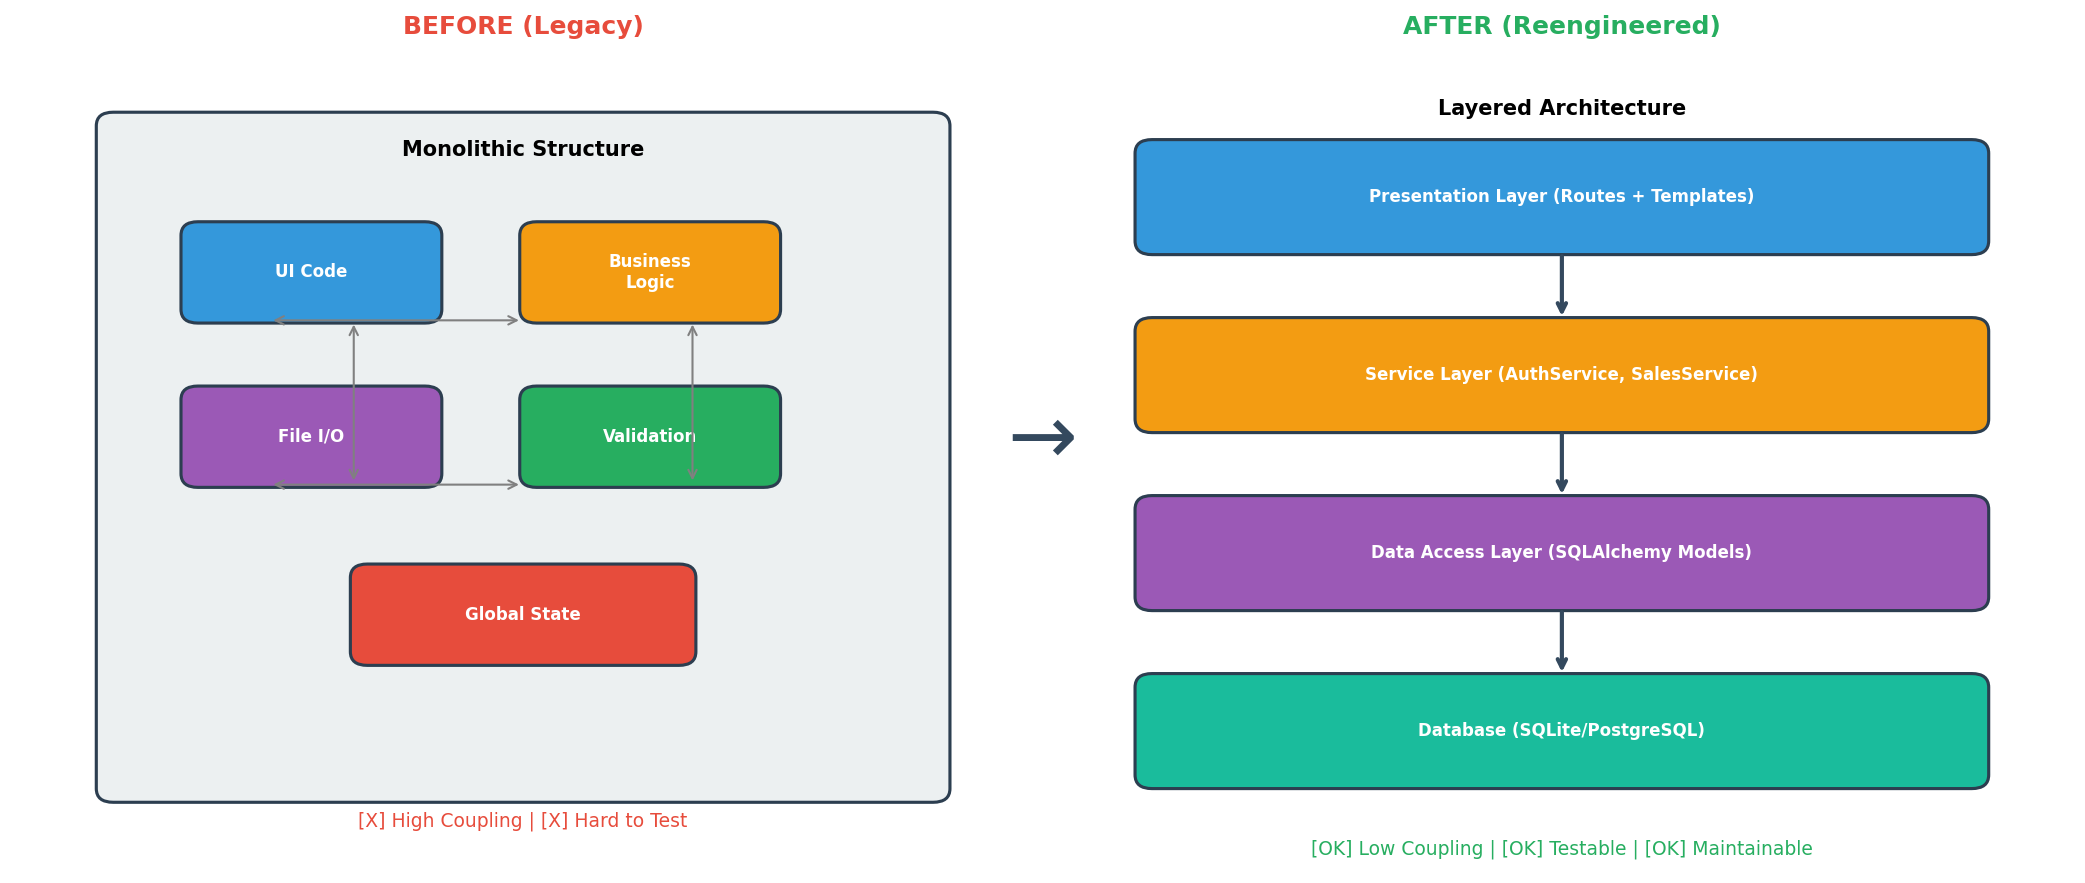
\includegraphics[width=0.95\textwidth]{images/code_restructuring.png}
  \caption{Code Restructuring Overview -- Transformation from monolithic
           structure to layered, modular architecture.}
  \label{fig:code-restructuring}
\end{figure}

\section{Refactoring Summary}

Table~\ref{tab:refactoring-summary} provides an overview of the proposed
refactorings to address the code smells identified in Chapter 2.

\begin{table}[h]
  \centering
  \caption{Refactoring Summary -- Smell to Solution Mapping}
  \label{tab:refactoring-summary}
  \begin{tabular}{p{1cm} p{3.5cm} p{4cm} p{4.5cm}}
    \toprule
    \textbf{Smell} & \textbf{Problem} & \textbf{Refactoring} & \textbf{Benefit} \\
    \midrule
    CS1 & Duplicated trees & Consolidate to single \texttt{src/} & Reduced maintenance \\
    CS2 & Scattered file I/O & Extract Repository pattern & Centralized data access \\
    CS3 & Magic numbers & Extract constants/config & Configurable, clear intent \\
    CS4 & Global mutable state & Introduce stateless services & Predictable behavior \\
    CS5 & Plaintext passwords & Hash with bcrypt & Security compliance \\
    CS6 & Poor error handling & Structured exception handling & Graceful degradation \\
    CS7 & God class & Single Responsibility split & Focused, testable classes \\
    \bottomrule
  \end{tabular}
\end{table}

\section{Proposed Refactorings (Legacy)}

\subsection*{Consolidate Duplicated Trees}

\begin{itemize}[leftmargin=1.2cm]
  \item Remove duplicate classes under \texttt{src/src/*}.
  \item Keep a single, clean \texttt{src/} tree with appropriate
        packages (e.g., \texttt{interfaces}, \texttt{bl}).
\end{itemize}

\subsection*{Relocate Forward-Engineered Code}

\begin{itemize}[leftmargin=1.2cm]
  \item Place all new web or API code under a dedicated directory
        (e.g., \texttt{forward-engineered/api},
        \texttt{forward-engineered/migration}), clearly separated from
        the legacy Java sources.
\end{itemize}

\subsection*{Extract Repositories from File I/O}

\begin{itemize}[leftmargin=1.2cm]
  \item Define repository interfaces such as:
        \texttt{InventoryRepository}, \texttt{EmployeeRepository},
        \texttt{RentalRepository}, \texttt{SalesRepository}.
  \item Implement text-backed adapters initially, then later swap to
        database-backed implementations with minimal impact on the
        business logic.
\end{itemize}

\subsection*{Encapsulate Business Rules}

\begin{itemize}[leftmargin=1.2cm]
  \item Introduce a \texttt{TransactionService} to handle tax,
        discounts, and late-fee calculations.
  \item Ensure UI controllers delegate to this service instead of
        embedding financial logic directly.
\end{itemize}

\subsection*{Improve Input Validation and Error Handling}

\begin{itemize}[leftmargin=1.2cm]
  \item Wrap user inputs (phone numbers, card numbers, etc.) in
        dedicated validators.
  \item Replace \texttt{Long.parseLong} loops and bare \texttt{try/catch}
        with robust error handling and user-friendly feedback.
\end{itemize}

\section{Before/After Illustrations}

The following examples demonstrate the concrete improvements achieved
through code restructuring.

\subsection{Sales Persistence Refactoring}

\textbf{Before} (direct file write scattered in \texttt{src/POS.java}):

\begin{lstlisting}[language=Java]
// POS.java - File I/O mixed with business logic
public void endPOS() {
    try {
        FileWriter fw2 = new FileWriter("Database/saleInvoiceRecord.txt", true);
        BufferedWriter bw2 = new BufferedWriter(fw2);
        
        bw2.write("Date: " + dateFormat.format(new Date()));
        bw2.newLine();
        bw2.write("Cashier: " + POSSystem.name);
        bw2.newLine();
        
        for (Item item : cart) {
            bw2.write(item.getName() + " x" + item.getQty() + " = $" + item.getTotal());
            bw2.newLine();
        }
        
        bw2.write("Total with tax: " + totalPrice);
        bw2.newLine();
        bw2.close();
    } catch (IOException e) {
        e.printStackTrace();  // Poor error handling
    }
}
\end{lstlisting}

\textbf{After} (clean service with repository abstraction):

\begin{lstlisting}[language=Python]
# services/sales_service.py - Clean separation of concerns
class SalesService:
    @staticmethod
    def complete_sale(sale_id, amount_paid, payment_method='Cash'):
        sale = Sale.query.get(sale_id)
        
        # Verify stock
        for sale_item in sale.items:
            if sale_item.item.quantity < sale_item.quantity:
                return False, f"Insufficient stock for {sale_item.item.name}"
        
        # Update inventory atomically
        for sale_item in sale.items:
            sale_item.item.update_quantity(sale_item.quantity, 'subtract')
        
        # Process payment
        sale.process_payment(amount_paid, payment_method)
        
        # Log activity
        ActivityLog.log(action='sale_completed', entity_id=sale.id)
        
        db.session.commit()
        return True, "Sale completed successfully"
\end{lstlisting}

\subsection{Authentication Refactoring}

\textbf{Before} (global state and plaintext passwords in \texttt{POSSystem.java}):

\begin{lstlisting}[language=Java]
// POSSystem.java - Security vulnerability
public static boolean logIn(String user, String pass) {
    for (Employee emp : employees) {
        if (emp.getId().equals(user) && emp.getPassword().equals(pass)) {
            username = user;     // Global mutable state
            password = pass;     // Plaintext password stored!
            role = emp.getRole();
            return true;
        }
    }
    return false;
}
\end{lstlisting}

\textbf{After} (stateless service with hashed passwords):

\begin{lstlisting}[language=Python]
# services/auth_service.py - Secure, stateless authentication
class AuthService:
    @staticmethod
    def authenticate(employee_id, password):
        employee = Employee.query.filter_by(
            employee_id=employee_id,
            is_active=True
        ).first()
        
        if not employee or not employee.check_password(password):
            return False, None, "Invalid credentials"
        
        # Log successful login for audit
        ActivityLog.log(
            action='login',
            employee_id=employee.id,
            ip_address=request.remote_addr
        )
        
        return True, employee, "Login successful"
\end{lstlisting}

\section{Restructuring Plan}

The restructuring plan is organised into phases:

\begin{itemize}[leftmargin=1.2cm]
  \item \textbf{Phase 1:} Directory cleanup and package declarations;
        remove \texttt{src/src/*} duplicates and normalise package
        names.
  \item \textbf{Phase 1.1:} Create and stabilise a dedicated
        \texttt{forward-engineered/} area for all new web or API code.
  \item \textbf{Phase 2:} Introduce repository interfaces and refactor
        legacy classes to call these repositories instead of using
        raw file I/O.
  \item \textbf{Phase 3:} Add services for business rules, implement
        unit tests around tax and late-fee calculations, and prepare the
        system for full data restructuring and migration.
\end{itemize}
